\documentclass{article}

\usepackage{iclr2020_conference,times}

% COMMENT for anonymous submission
% \def\nonanonymous{}

\ifdefined\nonanonymous
\iclrfinalcopy
\fi

% to avoid loading the natbib package, add option nonatbib:
%     \usepackage[nonatbib]{neurips_2019}

\usepackage[utf8]{inputenc} % allow utf-8 input
\usepackage[T1]{fontenc}    % use 8-bit T1 fonts
\usepackage{hyperref}       % hyperlinks
\usepackage{url}            % simple URL typesetting
\usepackage{booktabs}       % professional-quality tables
\usepackage{amsfonts}       % blackboard math symbols
\usepackage{nicefrac}       % compact symbols for 1/2, etc.
\usepackage{microtype}      % microtypography

% Not part of the offical NeurIPS template
\usepackage{amssymb}
\usepackage{amsthm}
\usepackage{bm}
\usepackage{mathtools}
\usepackage{caption}
\usepackage{subcaption}
\usepackage{caption}
\usepackage{csquotes}
\usepackage{layouts}
\usepackage{float}
\usepackage{todonotes}
\usepackage{enumitem}

% Algorithms
\usepackage{algorithm}
\usepackage[noend]{algpseudocode}
\algnewcommand{\Let}[2]{\State #1 $\gets$ #2}
\algrenewcommand\Call[2]{\textproc{#1}(#2)}

% Kabel Tables
\usepackage{multirow}
\usepackage{tabu}
\usepackage{longtable}
\captionsetup[table]{skip=5pt}

\let\cite\citep
\title{Neural Arithmetic Units}

% The \author macro works with any number of authors. There are two commands
% used to separate the names and addresses of multiple authors: \And and \AND.
%
% Using \And between authors leaves it to LaTeX to determine where to break the
% lines. Using \AND forces a line break at that point. So, if LaTeX puts 3 of 4
% authors names on the first line, and the last on the second line, try using
% \AND instead of \And before the third author name.

\author{%
  Andreas Madsen \\
  Computationally Demanding \\
  \texttt{amwebdk@gmail.com}
  \And
  Alexander Rosenberg Johansen \\
  Technical University of Denmark \\
  \texttt{aler@dtu.dk} \\
}

\begin{document}

\maketitle

\begin{abstract}

%Learning exact arithmetic operation of real numbers, as part of a neural network, presents a unique challenge. Neural networks can approximate complex functions by learning from labeled data. However, when extrapolating to out-of-distribution samples neural networks often fail. Learning the underlying logic, as opposed to an approximation, is crucial in applications that depends on inferring physical models, comparing, or counting as part of the model.

%Alternative
%What’s the domain?
Neural networks can approximate complex functions, but they struggle to perform exact arithmetic operations over real numbers.
%What’s the issue?
The lack of inductive bias for arithmetic operations leaves neural networks without the underlying logic needed to extrapolate on tasks such as addition, subtraction, and multiplication.
%What’s your contribution?
We present two new neural network components: the Neural Addition Unit (NAU), which can learn to add and subtract; and Neural Multiplication Unit (NMU) that can multiply subsets of a vector.
%Why is it novel?
The NMU is to our knowledge the first arithmetic neural network component that can learn multiplication of a vector with a large hidden size.
%What’s interesting about it?
The two new components draw inspiration from a theoretical analysis of recent arithmetic components.
We find that careful initialization, restricting parameter space, and regularizing for sparsity is important when optimizing the NAU and NMU.
%How does it perform?
Our results, compared with previous attempts, show that the NAU and NMU converges more consistently, have fewer parameters, learn faster, do not diverge with large hidden sizes, obtain sparse and meaningful weights, and can extrapolate to negative and small numbers.\ifdefined\nonanonymous\footnote{Implementation is available on GitHub: \url{https://github.com/AndreasMadsen/stable-nalu}.}\fi

%What’s the domain?
%Exact arithmetic operations of real numbers in Neural Networks present a unique learning challenge for machine learning models.
%What’s the issue?
%Neural networks can approximate complex functions by learning from labeled data. However, when extrapolating to out-of-distribution samples neural networks often fail. Learning the underlying logic, as opposed to an approximation, is crucial for applications such as comparing, counting, and inferring physical models.
%What’s your contribution?
%Our proposed Neural Addition Unit (NAU) and Neural Multiplication Unit (NMU) can learn, using backpropagation, the underlying rules of real number addition, subtraction, and multiplication thereby performing well when extrapolating.
%Why is it novel?
%The proposed units controls the arithmetic operation by using a sparse weight matrix, which allows the units to perform exact arithmetic operations.
%What’s interesting about it?
%Through theoretical analysis, supported by empirical evidence, we justify how the NAU and NMU improve over previous methods. Our experimental setting, motivated by previous work, includes an arithmetic extrapolation task and multiplication of up to 20 MNIST digits.
%How does it perform?
%We show that NAU and NMU have fewer parameters, converges more consistently, learns faster, handles large hidden sizes better, and have more meaningful discrete values than previous attempts.\ifdefined\nonanonymous\footnote{Implementation is available on GitHub: \url{https://github.com/AndreasMadsen/stable-nalu}.}\fi
\end{abstract}

\section{Introduction}
When studying intelligence, insects, reptiles, and humans have been found to possess neurons with the capacity to hold integers, real numbers, and perform arithmetic operations \cite{nieder-neuronal-number,rugani-arithmetic-chicks,gallistel-numbers-in-brain}.
In our quest to mimic intelligence, we have put much faith in neural networks, which in turn has provided unparalleled and often superhuman performance in tasks requiring high cognitive abilities \cite{natureGo,bert,openai-learning-dexterous}.
However, when using neural networks to solve simple arithmetic problems, such as counting, multiplication, or comparison, they systematically fail to extrapolate onto unseen ranges \cite{stillNotSystematic,suzgun2019evaluating,trask-nalu}.
The absence of inductive bias makes it difficult for neural networks to extrapolate well on arithmetic tasks as they lack the underlying logic to represent the required operations.

A neural component that can solve arithmetic problems should be able to: take an arbitrary hidden input, learn to select the appropriate elements, and apply the desired arithmetic operation.
A recent attempt to achieve this goal is the Neural Arithmetic Logic Unit (NALU) by \citet{trask-nalu}.

The NALU models the inductive bias explicitly via two sub-units: the $\text{NAC}_{+}$ for addition/subtraction and the $\text{NAC}_{\bullet}$ for multiplication/division.
The sub-units are softly gated between, using a sigmoid function, to exclusively select one of the sub-units.
However, we find that the soft gating-mechanism and the $\text{NAC}_{\bullet}$ are fragile and hard to learn.

In this paper, we analyze and improve upon the $\text{NAC}_{+}$ and $\text{NAC}_{\bullet}$ with respect to addition, subtraction, and multiplication.
Our proposed improvements, namely the Neural Addition Unit (NAU) and Neural Multiplication Unit (NMU), are more theoretically founded and improve performance regarding stability, speed of convergence, and interpretability of weights.
Most importantly, the NMU supports both negative and small numbers and a large hidden input-size, which is paramount as neural networks are overparameterized and hidden values are often unbounded.

The improvements, which are based on a theoretical analysis of the NALU and its components, are achieved by a simplification of the parameter matrix for a better gradient signal, a sparsity regularizer, and a new multiplication unit that can be optimally initialized.
The NMU does not support division.
However, we find that the $\text{NAC}_{\bullet}$ in practice also only supports multiplication and cannot learn division (theoretical analysis on division discussed in section \ref{sssec:nac-mul}).

To analyze the impact of each improvement, we introduce several variants of the $\text{NAC}_{\bullet}$.
We find that allowing division makes optimization for multiplication harder, linear and regularized weights improve convergence, and the NMU way of multiplying is critical when increasing the hidden size.

Furthermore, we improve upon existing benchmarks in \citet{trask-nalu} by expanding the ``simple function task'', expanding ``MNIST Counting and Arithmetic Tasks'' with a multiplicative task, and using an improved success-criterion \citet{maep-madsen-johansen-2019}.
This success-criterion is important because the arithmetic layers are solving a logical problem.
We propose the MNIST multiplication variant as we want to test the NMU’s and $\text{NAC}_{\bullet}$’s ability to learn from real data and extrapolate.

\begin{figure}[t]
\centering
\vspace{-1em}
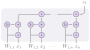
\includegraphics[scale=0.65]{graphics/nmu.pdf}
\caption{Visualization of NMU for a single output scalar $z_1$, this construction repeats for every element in the output vector $\mathbf{z}$.}
\end{figure}

\subsection{Learning a 10 parameter function}
Consider the static function $t = (x_1 + x_2) \cdot (x_1 + x_2 + x_3 + x_4)$ for $x \in \mathbb{R}^4$. To illustrate the ability of $\mathrm{NAC}_{\bullet}$, NALU, and our proposed NMU, we conduct 100 experiments for each model, where we attempt to fit this function. Table \ref{tab:very-simple-function-results} shows that NMU has a higher success rate and converge faster.
\begin{table}[!h]

\caption{\label{tab:very-simple-function-results}Comparison of the success-rate, when the model converged, and the sparsity error for all weight matrices, with 95\% confidence interval on the $t = (x_1 + x_2) \cdot (x_1 + x_2 + x_3 + x_4)$ task. Each value is a summary of 100 different seeds.}
\centering
\begin{tabular}{crllll}
\toprule
\multicolumn{1}{c}{Op} & \multicolumn{1}{c}{Model} & \multicolumn{1}{c}{Success} & \multicolumn{2}{c}{Solved at} & \multicolumn{1}{c}{Sparsity error} \\
\cmidrule(l{3pt}r{3pt}){1-1} \cmidrule(l{3pt}r{3pt}){2-2} \cmidrule(l{3pt}r{3pt}){3-3} \cmidrule(l{3pt}r{3pt}){4-5} \cmidrule(l{3pt}r{3pt}){6-6}
 &  & Rate & Median & Mean & Mean\\
\midrule
 & $\mathrm{NAC}_{\bullet}$ & $13\% {~}^{+8\%}_{-5\%}$ & $5.5 \cdot 10^{4}$ & $5.9 \cdot 10^{4} {~}^{+7.8 \cdot 10^{3}}_{-6.6 \cdot 10^{3}}$ & $7.5 \cdot 10^{-6} {~}^{+2.0 \cdot 10^{-6}}_{-2.0 \cdot 10^{-6}}$\\

\nopagebreak
 & NALU & $26\% {~}^{+9\%}_{-8\%}$ & $7.0 \cdot 10^{4}$ & $7.8 \cdot 10^{4} {~}^{+6.2 \cdot 10^{3}}_{-8.6 \cdot 10^{3}}$ & $9.2 \cdot 10^{-6} {~}^{+1.7 \cdot 10^{-6}}_{-1.7 \cdot 10^{-6}}$\\

\nopagebreak
\multirow{-3}{*}{\centering\arraybackslash $\bm{\times}$} & NMU & $\mathbf{94\%} {~}^{+3\%}_{-6\%}$ & $\mathbf{1.4 \cdot 10^{4}}$ & $\mathbf{1.4 \cdot 10^{4}} {~}^{+2.2 \cdot 10^{2}}_{-2.1 \cdot 10^{2}}$ & $\mathbf{2.6 \cdot 10^{-8}} {~}^{+6.4 \cdot 10^{-9}}_{-6.4 \cdot 10^{-9}}$\\
\bottomrule
\end{tabular}
\end{table}


\section{Introducing differentiable binary arithmetic operations}
\label{sec:Nalu}
Our goal is to achieve arithmetic operations between the elements of a vector. Such that the output is an addition, subtraction, multiplication, or division of arbitrary elements of a vector $\mathbf{x}$ (e.g. ${x_5 + x_1 \cdot x_7}$), which we formalize as
\begin{equation}
x_1\circ_1 x_2 \circ_2 \cdots x_{k-1} \circ_{k-1} x_{k}\ |\ (x_1, \dots, x_k) \in \mathbf{x}, \mathbf{x} \in \mathbb{R}^n, \circ_i \in \{+, -, \times, \div \}
\label{eq:goal}
\end{equation}
. The Neural Arithmetic Logic Unit (NALU) \cite{trask-nalu} attempts to solve equation \ref{eq:goal} by presenting two sub-units; the $\text{NAC}_{+}$ and $\text{NAC}_{\bullet}$ to exclusively represent either the $\{+, -\}$ or the $\{\times, \div \}$ operations.
The NALU attempts to have either $\text{NAC}_{+}$ or $\text{NAC}_{\bullet}$ selected exclusively, which could require the NALU to be applied multiple times (alternating between $\text{NAC}_{+}$ and $\text{NAC}_{\bullet}$) in order to represent the entire space of solutions for equation \ref{eq:goal}.

The $\text{NAC}_{+}$ and $\text{NAC}_{\bullet}$ are defined accordingly,
\begin{align}
W_{h_\ell, h_{\ell-1}} &= \tanh(\hat{W}_{h_\ell, h_{\ell-1}}) \sigma(\hat{M}_{h_\ell, h_{\ell-1}}) \label{eq:weight}\\
\textrm{NAC}_+:\ z_{h_\ell} &= \sum_{h_{\ell-1}=1}^{H_{\ell-1}} W_{h_{\ell}, h_{\ell-1}} z_{h_{\ell-1}} \label{eq:naca}\\
\textrm{NAC}_\bullet:\ z_{h_\ell} &= \exp\left(\sum_{h_{\ell-1}=1}^{H_{\ell-1}} W_{h_{\ell}, h_{\ell-1}} \label{eq:nacm}\log(|z_{h_{\ell-1}}| + \epsilon) \right)
\end{align}
where $\hat{\mathbf{W}}, \hat{\mathbf{M}} \in \mathbb{R}^{H_{\ell} \times H_{\ell-1}}$ are trainable weight matrices. The matrices are combined using tanh and sigmoid transformation to bias the parameters towards a $\{-1,0,1\}$ solution. Having $\{-1,0,1\}$ allows a linear layer to exactly emulate the binary $\{+, -\}$ operation between elements of a vector as used when computing the $\text{NAC}_{+}$.
The $\text{NAC}_{\bullet}$ extends the $\text{NAC}_{+}$ by using an exponential log transformation, which, with $\{-1,0,1\}$ weight values, becomes the $\{\times, \div \}$ operations (within $\epsilon$ precision).

The NALU combines these units with a gating mechanism $\mathbf{z} = \mathbf{g} \odot \text{NAC}_{+} + (1 - \mathbf{g}) \odot \text{NAC}_{\bullet}$ given $\mathbf{g} = \sigma(\mathbf{G} \mathbf{x})$. The idea is that the NALU should be a plug-and-play component in a neural network and has the ability to, with stochastic gradient descent and backpropagation, to learn the functionality in equation \ref{eq:goal}.

\subsection{Challenges of the $\text{NAC}_{+}$ and $\text{NAC}_{\bullet}$}
To simplify the problem we have chosen to leave out the gating mechanism and focus on the sub-units, assuming "oracle gating". We have not had any consistent success of convergence using the gating mechanism using the NALU or by combining our own proposed sub-units (NAU, NMU), as shown in table \ref{tab:function-task-static-defaults}. We find that gating between $\text{NAC}_{+}$ and $\text{NAC}_{\bullet}$ is challenging. This is likely due to the vastly different gradients, causing addition to be learned much faster than multiplication.

%In section \ref{sssec:weight} we analyse the gradients of equation \ref{eq:weight} and propose a cliped linear alternative, with a regularizer that biases towards $\{-1, 0, 1\}$. This results in an alternative addition unit called NAU.

%In section \ref{sssec:nac-mul} we analyse the gradient of $\text{NAC}_{\bullet}$, and propose an alternative construction called NMU, that has a more well-behaved loss space.

%In section \ref{sssec:nac-add-moments} we analyse the moments of $\text{NAC}_{+}$ and NAU, and derive the optimal weight initializations.

%In section \ref{sssec:nac-mul-moments} we analyse the moments of $\text{NAC}_{\bullet}$ and NMU, and show that the NMU have a more well-behaved expectation and variance. \todo{Maybe remove this overview?}

\subsubsection{Weight matrix construction}\label{sssec:weight}

The weight matrix construction $\mathrm{tahn}(\hat{W}_{h_{\ell-1},h_\ell}) \sigma(\hat{M}_{h_{\ell-1},h_\ell})$ has the properties that could make convergence challenging using gradient decent. Firstly, the loss gradient with respect to the weight matrices can be derived from equation \ref{eq:weight} (derivation in appendix \ref{sec:appendix:gradient-derivatives:weight-matrix-construction}).
\begin{equation}
\begin{aligned}
\frac{\partial \mathcal{L}}{\partial \hat{W}_{h_{\ell-1},h_\ell}} &= \frac{\partial \mathcal{L}}{\partial W_{h_{\ell-1},h_\ell}} (1 - \tanh^2(\hat{W}_{h_{\ell-1},h_\ell})) \sigma(\hat{M}_{h_{\ell-1},h_\ell}) \\
\frac{\partial \mathcal{L}}{\partial \hat{M}_{h_{\ell-1},h_\ell}} &= \frac{\partial \mathcal{L}}{\partial W_{h_{\ell-1},h_\ell}} \tanh(\hat{W}_{h_{\ell-1},h_\ell}) \sigma(\hat{M}_{h_{\ell-1},h_\ell}) (1 - \sigma(\hat{M}_{h_{\ell-1},h_\ell}))
\end{aligned}
\label{eq:nac-weight-gradient}
\end{equation}

For $E[\hat{W}_{h_{\ell-1},h_\ell}] = 0$, which is necessary to satisfy $E[z_{h_\ell}]  = 0$ that is a desired property  \cite{glorot-initialization}, the expectation of the $\hat{M}_{h_{\ell-1},h_\ell}$ gradient becomes zero.

Secondly, in our empirical analysis we find that equation \ref{eq:weight} does not create the desired bias for $\{-1, 0, 1\}$, as it fails to converge towards such values.

To create the desired bias of $\{-1, 0, 1\}$, we add a biasing regularizer $\mathcal{R}_{\ell,\mathrm{bias}}$. To prevent the gradient challenges of equation \ref{eq:nac-weight-gradient} we propose a simple clamped linear construction with an out-of-bound regularizer $\mathcal{R}_{\ell,\mathrm{oob}}$ to force $\hat{W}$ to be within $[-1, 1]$ and ensure that the gradient is always present. These regualizers are added to the loss function, $\mathcal{L} = \hat{\mathcal{L}} + \lambda_{\mathrm{bias}} \mathcal{R}_{\ell,\mathrm{bias}} + \lambda_{\mathrm{oob}} \mathcal{R}_{\ell,\mathrm{oob}}$.
\begin{align}
W_{h_{\ell-1},h_\ell} &= \min(\max(\hat{W}_{h_{\ell-1},h_\ell}, -1), 1), \\
\mathcal{R}_{\ell,\mathrm{bias}} &= \frac{1}{H_\ell + H_{\ell-1}} \sum_{h_\ell=1}^{H_\ell} \sum_{h_{\ell-1}=1}^{H_{\ell-1}} \hat{W}_{h_{\ell-1},h_\ell}^2 (1 - |\hat{W}_{h_{\ell-1},h_\ell}|)^2 \\
\mathcal{R}_{\ell,\mathrm{oob}} &= \frac{1}{H_\ell + H_{\ell-1}} \sum_{h_\ell=1}^{H_\ell} \sum_{h_{\ell-1}=1}^{H_{\ell-1}} \max(|\hat{W}_{h_{\ell-1},h_\ell}| - 1, 0)^2 \\
\textrm{NAU}:\ z_{h_\ell} &= \sum_{h_{\ell-1}=1}^{H_{\ell-1}} W_{h_{\ell}, h_{\ell-1}} z_{h_{\ell-1}}
\end{align}

\subsubsection{Challenges of division} \label{sssec:nac-mul}

The $\text{NAC}_{\bullet}$, as formulated in equation \ref{eq:nacm}, has the ability to learn exact multiplication and division of elements from a vector if the weights of $W_{h_{\ell-1},h_\ell}$ are one of $\{-1, 0, 1\}$.

However, backpropagation through the $\text{NAC}_{\bullet}$ unit (equation \ref{eq:dz}, derivation in Appendix \ref{sec:appendix:gradient-derivatives:gradient-nac-mul}) reveals that if $|z_{h_{\ell-1}}|$ is near zero, $W_{h_{\ell-1},h_\ell}$ is negative and $\epsilon$ is small, the gradient term will explode and oscillate between large positive and large negative values, which can be problematic in optimization \cite{adam-optimization}, as visualized in figure \ref{fig:nac-mul-eps-issue}.
\begin{align}
%\frac{\partial \mathcal{L}}{\partial W_{h_{\ell}, h_{\ell - 1}}} &= \frac{\partial \mathcal{L}}{\partial z_{h_\ell}} \frac{\partial z_{h_\ell}}{\partial W_{h_{\ell}, h_{\ell - 1}}} = \frac{\partial \mathcal{L}}{\partial z_{h_\ell}} z_{h_\ell} \log(|z_{h_{\ell-1}}| + \epsilon) \label{eq:dw}\\
\frac{\partial \mathcal{L}}{\partial z_{h_{\ell-1}}} &= \sum_{h_\ell = 1}^{H_\ell} \frac{\partial \mathcal{L}}{\partial z_{h_\ell}} \frac{\partial z_{h_\ell}}{\partial z_{h_{\ell-1}}} = \sum_{h_\ell = 1}^{H_\ell} \frac{\partial \mathcal{L}}{\partial z_{h_\ell}} z_{h_\ell} W_{h_\ell, h_{\ell-1}} \frac{\mathrm{sign}(z_{h_{\ell-1}})}{|z_{h_{\ell-1}}| + \epsilon}\label{eq:dz}
\end{align}

This is not an issue for positive values of $W_{h_{\ell-1},h_\ell}$ (multiplication), as $z_{h_{\ell}}$ and $z_{h_{\ell-1}}$ will be correlated causing the terms $z_{h_\ell}$ and $\frac{\mathrm{sign}(z_{h_{\ell-1}})}{|z_{h_{\ell-1}}| + \epsilon}$ to partially cancel out.

This gradient can be particular problematic when considering that $E[z_{h_{\ell-1}}] = 0$ is a desired property when initializing \cite{glorot-initialization}. An alternative multiplication operator must thus be able to not explode for $z_{h_{\ell-1}}$ near zero.

\begin{figure}[h]
\centering
\begin{subfigure}{.33\textwidth}
  \centering
  \includegraphics[width=\linewidth]{graphics/nac-mul-eps-1em7.png}
  \caption{$\mathrm{NAC}_{\bullet}$ with $\epsilon = 10^{-7}$}
\end{subfigure}%
\begin{subfigure}{.33\textwidth}
  \centering
  \includegraphics[width=\linewidth]{graphics/nac-mul-eps-1em1.png}
  \caption{$\mathrm{NAC}_{\bullet}$ with $\epsilon = 0.1$}
\end{subfigure}
%\begin{subfigure}{.33\textwidth}
%  \centering
%  \includegraphics[width=\linewidth]{graphics/nac-mul-eps-1.png}
%  \caption{$\epsilon = 1$}
%\end{subfigure}
\begin{subfigure}{.33\textwidth}
  \centering
\includegraphics[width=\linewidth]{graphics/nac-mul-nmu.png}
  \caption{Our NMU solution}
\end{subfigure}

\caption{RMS loss curvature for a $\mathrm{NAC}_{+}$ layer followed by either a $\mathrm{NAC}_{\bullet}$ or NMU layer. The weight matrices constrained are to $\mathbf{W}_1 = \left[\protect\begin{smallmatrix}
w_1 & w_1 & 0 & 0 \\
w_1 & w_1 & w_1 & w_1
\protect\end{smallmatrix}\right]$, $\mathbf{W}_2 = \left[\protect\begin{smallmatrix}
w_2 & w_2
\protect\end{smallmatrix}\right]$. The problem is $x = \left(1, 1.2, 1.8, 2\right), t = 13.2$. The desired solution is $w_1 = w_2 = 1$, although this problem have additional undesired solutions.}
\label{fig:nac-mul-eps-issue}
\end{figure}

\subsubsection{Initialization of $\mathrm{NAC}_{\bullet}$}
Initialization is important to consider for fast and consistent convergence, one desired property is that weights can be initialized such that $E[z_{h_\ell}] = 0$ \cite{glorot-initialization}. Using second order Taylor approximation and assuming all $z_{h_{\ell-1}}$ are uncorrelated, the expectation of $\mathrm{NAC}_{\bullet}$ can be estimated as
\begin{equation}
E[z_{h_\ell}] \approx \left(1 + \frac{1}{2} Var[W_{h_\ell, h_{\ell-1}}] \log(|E[z_{h_{\ell-1}}]| + \epsilon)^2\right)^{H_{\ell-1}} \Rightarrow E[z_{h_\ell}] > 1 \label{eq:nac-mul:expectation}
\end{equation}
As shown in equation \ref{eq:nac-mul:expectation}, satisfying $E[z_{h_\ell}] = 0$ for $\mathrm{NAC}_{\bullet}$ is likely impossible. The variance can also not be input-independent initialized, and is likely to explode (proofs in Appendix \ref{sec:appendix:moments:nac-mul}).

\subsubsection{Neural multiplication unit}
To solve the the gradient and initialization challenges for $\mathrm{NAC}_{\bullet}$ we propose a new neural multiplication unit (NMU):

\begin{align}
W_{h_{\ell-1},h_\ell} &= \min(\max(\hat{W}_{h_{\ell-1},h_\ell}, 0), 1), \\
\mathcal{R}_{\ell,\mathrm{bias}} &= \frac{1}{H_\ell + H_{\ell-1}} \sum_{h_\ell=1}^{H_\ell} \sum_{h_{\ell-1}=1}^{H_{\ell-1}} \hat{W}_{h_{\ell-1},h_\ell}^2 (1 - \hat{W}_{h_{\ell-1},h_\ell})^2 \\
\mathcal{R}_{\ell,\mathrm{oob}} &= \frac{1}{H_\ell + H_{\ell-1}} \sum_{h_\ell=1}^{H_\ell} \sum_{h_{\ell-1}=1}^{H_{\ell-1}} \max\left(\left|\hat{W}_{h_{\ell-1},h_\ell} - \frac{1}{2}\right| - \frac{1}{2}, 0\right)^2 \\
\textrm{NMU}:\ z_{h_\ell} &= \prod_{h_{\ell-1}=1}^{H_{\ell-1}} \left(W_{h_{\ell-1},h_\ell} z_{h_{\ell-1}} + 1 - W_{h_{\ell-1},h_\ell} \right) \label{eq:nmu-defintion}
\end{align}
This has regualizers similar to that of NAU, and has the multiplicative identity when $W_{h_{\ell-1},h_\ell}=0$. The NMU unit does not support division, but supporting division is likely infeasible as dividing by $z_{h_{\ell-1}}$ near zero would cause explosions for the forward and backward pass.
Furthermore, previous experiments using the NALU for division does not work well hence very little is lost with this modification \cite{trask-nalu}.
As opposed to the $\mathrm{NAC}_{\bullet}$, the NMU can represent input of both negative and positive $z_{h_{\ell-1}}$ values and is not $\epsilon$ dependent, which allows the NMU to extrapolate inputs that are negative or smaller than $\epsilon$.

The gradients with respect to the weight and input in the NMU are (see details in Appendix \ref{sec:appendix:gradient-derivatives:gradient-nmu}):
\begin{align}
\frac{\partial \mathcal{L}}{\partial W_{h_{\ell}, h_{\ell - 1}}} &= \frac{\partial \mathcal{L}}{\partial z_{h_\ell}} \frac{\partial z_{h_\ell}}{\partial W_{h_{\ell}, h_{\ell - 1}}} = \frac{\partial \mathcal{L}}{\partial z_{h_\ell}} \frac{z_{h_\ell}}{W_{h_{\ell-1},h_\ell} z_{h_{\ell-1}} + 1 - W_{h_{\ell-1},h_\ell}} \left(z_{h_{\ell-1}} - 1\right) \label{eq:nmugrad-1} \\
\frac{\partial \mathcal{L}}{\partial z_{h_{\ell-1}}} &= \sum_{h_\ell = 1}^{H_\ell} \frac{\partial \mathcal{L}}{\partial z_{h_\ell}} \frac{\partial z_{h_\ell}}{\partial z_{h_{\ell-1}}} = \sum_{h_\ell = 1}^{H_\ell} \frac{z_{h_\ell}}{W_{h_{\ell-1},h_\ell} z_{h_{\ell-1}} + 1 - W_{h_{\ell-1},h_\ell}} W_{h_{\ell-1},h_\ell} \label{eq:nmugrad-2}
\end{align}

Note that the fraction in equation \ref{eq:nmugrad-1} and \ref{eq:nmugrad-2} does not explode for $z_{h_{\ell-1}}$ close to zero because the denominator cancels out the term for $h_{\ell-1}$ in $z_{h_\ell}$, as seen in equation \ref{eq:nmu-defintion}.

\subsubsection{Moments and initialization}
Our proposed NAU can be initialized using Glorot initialization as it is a linear layer. The $\mathrm{NAC}_{+}$ unit can also achieve an ideal initialization, although it is less trivial (details in Appendix \ref{sec:appendix:moments:weight-matrix-construction}).

Our proposed NMU is initialized with $E[W_{h_{\ell}, h_{\ell - 1}}] = \nicefrac{1}{2}$. Assuming all $z_{h_{\ell-1}}$ are uncorrelated, and $E[z_{h_{\ell-1}}] = 0$, which is the case for most units, the expectation can be approximated to
\begin{equation}
E[z_{h_\ell}] \approx \left(\frac{1}{2}\right)^{H_{\ell-1}}
\end{equation}
, this approaches zero for $H_{\ell-1} \rightarrow \infty$ (proof in Appendix \ref{sec:appendix:moments:nmu}). The NMU can, with the assumption that, $Var[z_{h_{\ell-1}}] = 1$ and $H_{\ell-1}$ is large, be initialized optimally with $Var[W_{h_{\ell-1},h_\ell}] = \frac{1}{4}$ (proof in Appendix \ref{sec:appendix:moments:nmu:initialization}). 
\section{Related work}
Pure neural models that learns arithmetic tasks through backpropagation have previously been attempted.
They either utilize convolutions, gating, differentiable memory, and/or attention architectures \cite{NeuralGPU,GridLSTM,NTM}.
Some of the results have close to perfect extrapolation. However, the models are constrained to work only on whole numbers and requires well defined arithmetic setups such as binary representations of numbers for input and output.
We do not test the expressiveness of current approximate approaches, but instead develop a fundamental new unit of computation with weight constraints to learn exact arithmetic operations that works on real numbers, without any assumptions of binary representations.

To handle operations on real numbers, the Neural Arithmetic Expression Calculator \cite{NAEC} propose learning the individual components needed.
They repeatedly combine program induction with a memory-encoder-decoder architecture trained with reinforcement learning.
While this model has the ability to dynamically handle a larger variety of expressions compared to our solution, they do not generalize much beyond interpolation length.

We use the NAU to do a subset-selection, which is then followed by either a summation or multiplication, in order to combine information from the input vector.
An alternative, fully differentiable version, is to use a gumbel-softmax to perform exact subset-selection \cite{DSS}.
This, however, has the restriction of having to use a predefined size of the subset, which is a strong assumption that our units are not limited by.

\section{Results}

\subsection{Simple function}

\begin{figure}[H]
\centering
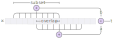
\includegraphics[scale=1]{graphics/function_task_static_problem.pdf}
\caption{Lorem Ipsum.}
\end{figure}

\subsubsection{Simple multiplication task}
\begin{table}[!h]

\caption{\label{tab:very-simple-function-results}Comparison of the success-rate, when the model converged, and the sparsity error for all weight matrices, with 95\% confidence interval on the $t = (x_1 + x_2) \cdot (x_1 + x_2 + x_3 + x_4)$ task. Each value is a summary of 100 different seeds.}
\centering
\begin{tabular}{crllll}
\toprule
\multicolumn{1}{c}{Op} & \multicolumn{1}{c}{Model} & \multicolumn{1}{c}{Success} & \multicolumn{2}{c}{Solved at} & \multicolumn{1}{c}{Sparsity error} \\
\cmidrule(l{3pt}r{3pt}){1-1} \cmidrule(l{3pt}r{3pt}){2-2} \cmidrule(l{3pt}r{3pt}){3-3} \cmidrule(l{3pt}r{3pt}){4-5} \cmidrule(l{3pt}r{3pt}){6-6}
 &  & Rate & Median & Mean & Mean\\
\midrule
 & $\mathrm{NAC}_{\bullet}$ & $13\% {~}^{+8\%}_{-5\%}$ & $5.5 \cdot 10^{4}$ & $5.9 \cdot 10^{4} {~}^{+7.8 \cdot 10^{3}}_{-6.6 \cdot 10^{3}}$ & $7.5 \cdot 10^{-6} {~}^{+2.0 \cdot 10^{-6}}_{-2.0 \cdot 10^{-6}}$\\

\nopagebreak
 & NALU & $26\% {~}^{+9\%}_{-8\%}$ & $7.0 \cdot 10^{4}$ & $7.8 \cdot 10^{4} {~}^{+6.2 \cdot 10^{3}}_{-8.6 \cdot 10^{3}}$ & $9.2 \cdot 10^{-6} {~}^{+1.7 \cdot 10^{-6}}_{-1.7 \cdot 10^{-6}}$\\

\nopagebreak
\multirow{-3}{*}{\centering\arraybackslash $\bm{\times}$} & NMU & $\mathbf{94\%} {~}^{+3\%}_{-6\%}$ & $\mathbf{1.4 \cdot 10^{4}}$ & $\mathbf{1.4 \cdot 10^{4}} {~}^{+2.2 \cdot 10^{2}}_{-2.1 \cdot 10^{2}}$ & $\mathbf{2.6 \cdot 10^{-8}} {~}^{+6.4 \cdot 10^{-9}}_{-6.4 \cdot 10^{-9}}$\\
\bottomrule
\end{tabular}
\end{table}


\subsubsection{Static function task - defaults}
% latex table generated in R 3.4.3 by xtable 1.8-3 package
% Fri May 10 17:19:56 2019
\begin{table}[H]
\centering
\caption{Shows the sucess-rate for extrapolation < $\epsilon$, at what global step the model converged at, and the sparse error for all weight matrices.} 
\begin{tabular}{lll |rrr}
  \hline
                      &                            & & \multicolumn{1}{l}{          converged.at} & \multicolumn{1}{l}{          sparse.error} & \multicolumn{1}{l}{          success.rate} \\ 
  operation            & model                      &     & \multicolumn{1}{l}{                      } & \multicolumn{1}{l}{                      } & \multicolumn{1}{l}{                      } \\ 
   \hline
  ${a \cdot b}$        & ${\mathrm{NAC}_\bullet}$ &     & $3371250$             & $8.0 \times 10^{-5}$ & $40\%$               \\ 
                       & NALU                       &     & ---                   &      ---              & $0\%$                   \\ 
                       & NMU                        &     & $1571900$             & $1.6 \times 10^{-4}$ & $100\%$              \\ \hline
  $a - b$              & ${\mathrm{NAC}_{+}}$      &     & $6300$                & $1.1 \times 10^{-1}$ & $100\%$              \\ 
                       & linear                     &     & $3300$                & $7.6 \times 10^{-2}$ & $100\%$              \\ 
                       & NALU                       &     & $1963250$             & $9.1 \times 10^{-2}$ & $40\%$               \\ 
                       & NAU                        &     & $3700$                & $4.3 \times 10^{-4}$ & $100\%$              \\ \hline 
  $a + b$              & ${\mathrm{NAC}_{+}}$      &     & $42900$               & $1.4 \times 10^{-1}$ & $100\%$              \\ 
                       & linear                     &     & $21300$               & $1.9 \times 10^{-1}$ & $100\%$              \\ 
                       & NALU                       &     & $81000$               & $1.9 \times 10^{-1}$ & $10\%$               \\ 
                       & NAU                        &     & $15500$               & $1.1 \times 10^{-4}$ & $100\%$              \\ 
   \hline
\end{tabular}
\end{table}


\subsubsection{Static function task - boundary}
\begin{figure}[H]
\centering
\includegraphics[width=\linewidth]{results/simple_function_static_input_size.pdf}
\caption{Lorem Ipsum.}
\end{figure}

\begin{figure}[H]
\centering
\includegraphics[width=\linewidth]{results/simple_function_static_overlap.pdf}
\caption{Lorem Ipsum.}
\end{figure}

\begin{figure}[H]
\centering
\includegraphics[width=\linewidth]{results/simple_function_static_subset.pdf}
\caption{Lorem Ipsum.}
\end{figure}

\subsection{sequential MNIST}

\begin{figure}[H]
\centering
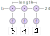
\includegraphics[scale=1]{graphics/mnist_sequence_problem.pdf}
\caption{Lorem Ipsum.}
\end{figure}


\section{Conclusion}

% Far better sucess-rate, learns faster, have discrete weights.
% NAC-mul, converges only 13% of the time on a very simple problem. Our NMU converges 94% of the time.
% We tested on a range of different dataset configurations and shown that this is generally the case.

% NMU, understands negative inputs and thus can extrapolate into that domain.
% NAU, produces discrete weights unlike NAC.

% The models are theoretically inspired.

% MNIST findings?

\clearpage
\ifdefined\nonanonymous
\subsubsection*{Acknowledgments}
We would like to thank Andrew Trask and the other authors of the NALU paper, for highlighting the importance and challenges of extrapolation in Neural Networks. We would also like to thank the students Raja Shan Zaker Kreen and William Frisch Møller from The Technical University of Denmark, who initially showed us that the NALU do not converge consistently. 

This research is funded by the Innovation Foundation Denmark through the DABAI project.
\fi

\bibliographystyle{iclr2020_conference}
\bibliography{bibliography}

\newpage
\appendix
\section{Gradient derivatives}

\subsection{Weight matrix construction}

The gradient of the weight matrix construction $\mathrm{tahn}({\hat{\mathbf{W}}}) \sigma({\hat{\mathbf{M}}})$ is straight forward to derive.



\begin{equation}
\begin{aligned}
\frac{\partial\mathcal{L}}{\partial \hat{W}_{h_\ell, h_{\ell-1}}} &= \frac{\partial\mathcal{L}}{\partial W_{h_\ell, h_{\ell-1}}} \frac{\partial W_{h_\ell, h_{\ell-1}}}{\partial \hat{W}_{h_\ell, h_{\ell-1}}} \\
&= \frac{\partial\mathcal{L}}{\partial W_{h_\ell, h_{\ell-1}}} (1 - \tanh^2(\hat{W}_{h_\ell, h_{\ell-1}})) \sigma(\hat{M}_{h_\ell, h_{\ell-1}}) \\
\frac{\partial\mathcal{L}}{\partial \hat{M}_{h_\ell, h_{\ell-1}}} &= \frac{\partial\mathcal{L}}{\partial W_{h_\ell, h_{\ell-1}}} \frac{\partial W_{h_\ell, h_{\ell-1}}}{\partial \hat{M}_{h_\ell, h_{\ell-1}}} \\
&= \frac{\partial\mathcal{L}}{\partial W_{h_\ell, h_{\ell-1}}} \tanh(\hat{W}_{h_\ell, h_{\ell-1}}) \sigma(\hat{M}_{h_\ell, h_{\ell-1}}) (1 - \sigma(\hat{M}_{h_\ell, h_{\ell-1}}))
\end{aligned}
\end{equation}

\subsection{Multiplication gradient}

\begin{equation}
\begin{aligned}
\frac{\partial z_{h_\ell}}{\partial W_{h_\ell, h_{\ell-1}}} &= \exp\left(\sum_{h'_{\ell-1}=1}^{H_{\ell-1}} W_{h_{\ell}, h'_{\ell-1}} \log(|z_{h'_{\ell-1}}| + \epsilon) \right) \log(|z_{h_{\ell-1}}| + \epsilon)
\end{aligned}
\end{equation}
\clearpage
\section{Moments}

\subsection{Expectation and variance for weight matrix construction in NAC layers}

The weight matrix construction in NAC, is defined in scalar notation as: 
\begin{equation}
W_{h_\ell, h_{\ell-1}} = \tanh(\hat{W}_{h_\ell, h_{\ell-1}}) \sigma(\hat{M}_{h_\ell, h_{\ell-1}})
\end{equation}

Simplifying the notation of this, and re-expressing it using stochastic variables with uniform distributions this can be written as:
\begin{equation}
\begin{aligned}
W &\sim \tanh(\hat{W}) \sigma(\hat{M}) \\
\hat{W} &\sim ~ U[-r, r] \\
\hat{M} &\sim ~ U[-r, r] 
\end{aligned}
\end{equation}

Since $\tanh({\hat{W}})$ is an odd-function and $E[\hat{W}] = 0$, deriving the expectation $E[W]$ is trivial.
\begin{equation}
\mathrm{E}[W] = \mathrm{E}[\tanh(\hat{W})]\mathrm{E}[\sigma(\hat{M})] = 0 \cdot \mathrm{E}[\sigma(\hat{M})] = 0
\end{equation}

The variance is more complicated, however as $\hat{W}$ and $\hat{M}$ are independent, it can be simplified to:
\begin{equation}
\mathrm{Var}[W] = \mathrm{E}[\tanh(\hat{W})^2] \mathrm{E}[\sigma(\hat{M})^2] - \mathrm{E}[\tanh(\hat{W})]^2 \mathrm{E}[\sigma(\hat{M})]^2 = \mathrm{E}[\tanh(\hat{W})^2] \mathrm{E}[\sigma(\hat{M})^2]
\end{equation}

These second moments can be analyzed independently. First for $\mathrm{E}[\tanh(\hat{W})^2]$:
\begin{equation}
\begin{aligned}
\mathrm{E}[\tanh(\hat{W})^2] &= \int_{-\infty}^{\infty} \tanh(x)^2 f_{U[-r, r]}(x)\ \mathrm{d}x \\
&= \frac{1}{2r} \int_{-r}^{r} \tanh(x)^2\ \mathrm{d}x \\
&= \frac{1}{2r} \cdot 2 \cdot (r - \tanh(r)) \\
&= 1 - \frac{\tanh(r)}{r}
\end{aligned}
\end{equation}

Then for $\mathrm{E}[\tanh(\hat{M})^2]$:
\begin{equation}
\begin{aligned}
\mathrm{E}[\sigma(\hat{M})^2] &= \int_{-\infty}^{\infty} \sigma(x)^2 f_{U[-r, r]}(x)\ \mathrm{d}x \\
&= \frac{1}{2r} \int_{-r}^{r} \sigma(x)^2\ \mathrm{d}x \\
&= \frac{1}{2r} \left(r - \tanh\left(\frac{r}{2}\right)\right)
\end{aligned}
\end{equation}

Finally this gives the variance:
\begin{equation}
\mathrm{Var}[W] = \frac{1}{2r} \left(1 - \frac{\tanh(r)}{r}\right) \left(r - \tanh\left(\frac{r}{2}\right)\right)
\end{equation}

\subsection{Expectation and variance of $\mathrm{NAC}_{\bullet}$}
\subsubsection{Forward pass}
Assuming that each $z_{h_{\ell-1}}$ are independent the expectation can be simplified to:
\begin{equation}
\begin{aligned}
E[z_{h_\ell}] &= E\left[\exp\left(\sum_{h_{\ell-1}=1}^{H_{\ell-1}} W_{h_{\ell}, h_{\ell-1}} \log(|z_{h_{\ell-1}}| + \epsilon) \right)\right] \\
&= E\left[\prod_{h_{\ell-1}=1}^{H_{\ell-1}} \exp(W_{h_{\ell}, h_{\ell-1}} \log(|z_{h_{\ell-1}}| + \epsilon)) \right] \\
&= \prod_{h_{\ell-1}=1}^{H_{\ell-1}} E[\exp(W_{h_{\ell}, h_{\ell-1}} \log(|z_{h_{\ell-1}}| + \epsilon))] \\
&= E[\exp(W_{h_{\ell}, h_{\ell-1}} \log(|z_{h_{\ell-1}}| + \epsilon))]^{H_{\ell-1}} \\
&= E\left[(|z_{h_{\ell-1}}| + \epsilon)^{W_{h_{\ell}, h_{\ell-1}}}\right]^{H_{\ell-1}} \\
&= E\left[f(z_{h_{\ell-1}}, W_{h_{\ell}, h_{\ell-1}})\right]^{H_{\ell-1}}
\end{aligned}
\end{equation}

Here we define $f$ as a non-linear transformation function of two independent stocastic variables:
\begin{equation}
f(z_{h_{\ell-1}}, W_{h_{\ell}, h_{\ell-1}}) = (|z_{h_{\ell-1}}| + \epsilon)^{W_{h_{\ell}, h_{\ell-1}}}
\end{equation}

We then take the second order taylor approximation of $f$, around $(E[z_{h_{\ell-1}}], E[W_{h_{\ell}, h_{\ell-1}}])$.
\begin{equation}
\begin{aligned}
&E[f(z_{h_{\ell-1}}, W_{h_{\ell}, h_{\ell-1}})] \approx
E\Bigg[\\
&f(E[z_{h_{\ell-1}}], E[W_{h_{\ell}, h_{\ell-1}}])\\
&+ \begin{bmatrix}
z_{h_{\ell-1}} - E[z_{h_{\ell-1}}] \\ W_{h_{\ell}, h_{\ell-1}} - E[W_{h_{\ell}, h_{\ell-1}}]
\end{bmatrix}^T \begin{bmatrix}
\frac{\partial f(z_{h_{\ell-1}}, W_{h_{\ell}, h_{\ell-1}})}{\partial z_{h_{\ell-1}}} \\
\frac{\partial f(z_{h_{\ell-1}}, W_{h_{\ell}, h_{\ell-1}})}{\partial W_{h_{\ell}, h_{\ell-1}}}
\end{bmatrix} \Bigg\rvert_{
\begin{cases}
z_{h_{\ell-1}} = E[z_{h_{\ell-1}}] \\
W_{h_{\ell}, h_{\ell-1}} = E[W_{h_{\ell}, h_{\ell-1}}]
\end{cases}
} \\
&+ \frac{1}{2} \begin{bmatrix}
z_{h_{\ell-1}} - E[z_{h_{\ell-1}}] \\ W_{h_{\ell}, h_{\ell-1}} - E[W_{h_{\ell}, h_{\ell-1}}]
\end{bmatrix}^T \\
&\bullet \begin{bmatrix}
\frac{\partial^2 f(z_{h_{\ell-1}}, W_{h_{\ell}, h_{\ell-1}})}{\partial^2 z_{h_{\ell-1}}} & \frac{\partial^2 f(z_{h_{\ell-1}}, W_{h_{\ell}, h_{\ell-1}})}{\partial z_{h_{\ell-1}} \partial W_{h_{\ell}, h_{\ell-1}}} \\
\frac{\partial^2 f(z_{h_{\ell-1}}, W_{h_{\ell}, h_{\ell-1}})}{\partial z_{h_{\ell-1}} \partial W_{h_{\ell}, h_{\ell-1}}} & \frac{\partial^2 f(z_{h_{\ell-1}}, W_{h_{\ell}, h_{\ell-1}})}{\partial^2 W_{h_{\ell}, h_{\ell-1}}}
\end{bmatrix} \Bigg\rvert_{
\begin{cases}
z_{h_{\ell-1}} = E[z_{h_{\ell-1}}] \\
W_{h_{\ell}, h_{\ell-1}} = E[W_{h_{\ell}, h_{\ell-1}}]
\end{cases}
} \\
&\bullet \begin{bmatrix}
z_{h_{\ell-1}} - E[z_{h_{\ell-1}}] \\ W_{h_{\ell}, h_{\ell-1}} - E[W_{h_{\ell}, h_{\ell-1}}]
\end{bmatrix}\Bigg]
\end{aligned}
\end{equation}

Because $E[z_{h_{\ell-1}} - E[z_{h_{\ell-1}}]] = 0$, $E[W_{h_{\ell}, h_{\ell-1}} - E[W_{h_{\ell}, h_{\ell-1}}]] = 0$, and $Cov[z_{h_{\ell-1}}, W_{h_{\ell}, h_{\ell-1}}] = 0$. This similifies to:
\begin{equation}
\begin{aligned}
&E[f(z_{h_{\ell-1}}, W_{h_{\ell}, h_{\ell-1}})] \approx
f(E[z_{h_{\ell-1}}], E[W_{h_{\ell}, h_{\ell-1}}])\\
&+ \frac{1}{2} Var\begin{bmatrix}
z_{h_{\ell-1}} \\ W_{h_{\ell}, h_{\ell-1}}
\end{bmatrix}^T \begin{bmatrix}
\frac{\partial^2 f(z_{h_{\ell-1}}, W_{h_{\ell}, h_{\ell-1}})}{\partial^2 z_{h_{\ell-1}}} \\
\frac{\partial^2 f(z_{h_{\ell-1}}, W_{h_{\ell}, h_{\ell-1}})}{\partial^2 W_{h_{\ell}, h_{\ell-1}}}
\end{bmatrix} \Bigg\rvert_{
\begin{cases}
z_{h_{\ell-1}} = E[z_{h_{\ell-1}}] \\
W_{h_{\ell}, h_{\ell-1}} = E[W_{h_{\ell}, h_{\ell-1}}]
\end{cases}
}
\end{aligned}
\end{equation}

Inserting the derivatives and computing the inner products yields:
\begin{equation}
\begin{aligned}
&E[f(z_{h_{\ell-1}}, W_{h_{\ell}, h_{\ell-1}})] \approx
(|E[z_{h_{\ell-1}}]| + \epsilon)^{E[W_{h_{\ell}, h_{\ell-1}}]} \\
&+ \frac{1}{2} Var[z_{h_{\ell-1}}] (|E[z_{h_{\ell-1}}]| + \epsilon)^{E[W_{h_{\ell}, h_{\ell-1}}] - 2} E[W_{h_{\ell}, h_{\ell-1}}] (E[W_{h_{\ell}, h_{\ell-1}}] - 1) \\
&+ \frac{1}{2} Var[W_{h_{\ell}, h_{\ell-1}}] (|E[z_{h_{\ell-1}}]| + \epsilon)^{E[W_{h_{\ell}, h_{\ell-1}}]} \log(|E[z_{h_{\ell-1}}]| + \epsilon)^2 \\
&=1 + \frac{1}{2} Var[W_{h_{\ell}, h_{\ell-1}}] \log(|E[z_{h_{\ell-1}}]| + \epsilon)^2
\end{aligned}
\end{equation}

This gives the final expectation:
\begin{equation}
\begin{aligned}
E[z_{h_\ell}] &= E\left[f(z_{h_{\ell-1}}, W_{h_{\ell}, h_{\ell-1}})\right]^{H_{\ell-1}} \\
&\approx\left(1 + \frac{1}{2} Var[W_{h_{\ell}, h_{\ell-1}}] \log(|E[z_{h_{\ell-1}}]| + \epsilon)^2\right)^{H_{\ell-1}}
\end{aligned}
\end{equation}

As this expectation is of particular interrest, we evaluate the error of the approximation, where $W_{h_{\ell}, h_{\ell-1}} \sim U[-r_w,r_w]$ and $z_{h_{\ell-1}} \sim U[0, r_z]$. These distributions are what is used in the simple function task is done.  The result is seen in figure \ref{fig:nac-mul-expectation-estimate}.
\begin{figure}[h]
\centering
\includegraphics[width=\linewidth]{graphics/nac-mul-expectation-estimate.pdf}
\caption{Error between theoretical approximation and the numerical approximation estimated by random sampling of $100000$ observations at each combination of $r_z$ and $r_w$.}
\label{fig:nac-mul-expectation-estimate}
\end{figure}

The variance can be derived using the same assumptions about expectation and no correlation.
\begin{equation}
\begin{aligned}
Var[z_{h_\ell}] &= E[z_{h_\ell}^2] - E[z_{h_\ell}]^2 \\
&= E\left[\prod_{h_{\ell-1}=1}^{H_{\ell-1}} (|z_{h_{\ell-1}}| + \epsilon)^{2 \cdot W_{h_{\ell}, h_{\ell-1}}} \right]
- E\left[\prod_{h_{\ell-1}=1}^{H_{\ell-1}} (|z_{h_{\ell-1}}| + \epsilon)^{W_{h_{\ell}, h_{\ell-1}}}\right]^2 \\
&= E\left[f(z_{h_{\ell-1}}, 2 \cdot W_{h_{\ell}, h_{\ell-1}}) \right]^{H_{\ell-1}}
- E\left[f(z_{h_{\ell-1}}, W_{h_{\ell}, h_{\ell-1}})\right]^{2\cdot H_{\ell-1}}
\end{aligned}
\end{equation}

We already have from the expectation result that:
\begin{equation}
E\left[f(z_{h_{\ell-1}}, W_{h_{\ell}, h_{\ell-1}})\right] \approx 1 + \frac{1}{2} Var[W_{h_{\ell}, h_{\ell-1}}] \log(|E[z_{h_{\ell-1}}]| + \epsilon)^2
\end{equation}

By substitution of variable we have that:
\begin{equation}
\begin{aligned}
E\left[f(z_{h_{\ell-1}}, 2 \cdot W_{h_{\ell}, h_{\ell-1}})\right] &\approx 1 + \frac{1}{2} Var[2 \cdot W_{h_{\ell}, h_{\ell-1}}] \log(|E[z_{h_{\ell-1}}]| + \epsilon)^2 \\
&= \approx 1 + 2 \cdot Var[W_{h_{\ell}, h_{\ell-1}}] \log(|E[z_{h_{\ell-1}}]| + \epsilon)^2
\end{aligned}
\end{equation}

This gives the variance:
\begin{equation}
\begin{aligned}
Var[z_{h_\ell}] &= E\left[f(z_{h_{\ell-1}}, 2 \cdot W_{h_{\ell}, h_{\ell-1}}) \right]^{H_{\ell-1}}
- E\left[f(z_{h_{\ell-1}}, W_{h_{\ell}, h_{\ell-1}})\right]^{2\cdot H_{\ell-1}} \\
&\approx \left(1 + 2 \cdot Var[W_{h_{\ell}, h_{\ell-1}}] \log(|E[z_{h_{\ell-1}}]| + \epsilon)^2\right)^{H_{\ell-1}} \\
&- \left(1 + \frac{1}{2} \cdot Var[W_{h_{\ell}, h_{\ell-1}}] \log(|E[z_{h_{\ell-1}}]| + \epsilon)^2\right)^{2\cdot H_{\ell-1}}
\end{aligned}
\end{equation}

\subsubsection{Backward pass}

The expectation of the backpropagation term:
\begin{equation}
E[\delta_{h_\ell}] = E\left[\sum_{h_{\ell+1}=1}^{H_{\ell+1}} \delta_{h_{\ell+1}} \frac{\partial z_{h_{\ell+1}}}{\partial z_{h_\ell}}\right] = H_{\ell+1} E[\delta_{h_{\ell+1}}] E\left[\frac{\partial z_{h_{\ell+1}}}{\partial z_{h_\ell}}\right]
\end{equation}

Where we have that:
\begin{equation}
E\left[\frac{\partial z_{h_{\ell+1}}}{\partial z_{h_\ell}}\right] = E[{h_{\ell+1}}] E[W_{h_{\ell+1}, h_{\ell}}] E\left[ \frac{\mathrm{abs}'(z_{h_{\ell}})}{|z| + \epsilon}\right] = E[m_{h_{\ell+1}}] \cdot 0 \cdot E\left[ \frac{\mathrm{abs}'(z_{h_{\ell}})}{|z| + \epsilon}\right] = 0
\end{equation}

Deriving the variance is more complicated as:
\begin{equation}
\begin{aligned}
Var\left[\frac{\partial m_{h_{\ell+1}}}{\partial z_{h_\ell}}\right] &= Var\left[m_{h_{\ell+1}} W_{h_{\ell+1}, h_{\ell}} \frac{\mathrm{abs}'(z_{h_{\ell}})}{|z_{h_{\ell}}| + \epsilon}\right]
\end{aligned}
\end{equation}

Assuming independence between each term this can be simplified to as:
\begin{equation}
\begin{aligned}
Var\left[\frac{\partial z_{h_{\ell+1}}}{\partial z_{h_\ell}}\right] &= E[z_{h_{\ell+1}}^2] E[W_{h_{\ell+1}, h_{\ell}}^2] E\left[\left( \frac{\mathrm{abs}'(z_{h_{\ell}})}{|z_{h_{\ell}}| + \epsilon}\right)^2\right] \\
&- E[z_{h_{\ell+1}}]^2 E[W_{h_{\ell+1}, h_{\ell}}]^2 E\left[ \frac{\mathrm{abs}'(z_{h_{\ell}})}{|z_{h_{\ell}}| + \epsilon}\right]^2 \\
&= E[z_{h_{\ell+1}}^2] Var[W_{h_{\ell+1}, h_{\ell}}] E\left[\left( \frac{\mathrm{abs}'(z_{h_{\ell}})}{|z_{h_{\ell}}| + \epsilon}\right)^2\right] \\
&- E[z_{h_{\ell+1}}]^2 \cdot 0 \cdot E\left[ \frac{\mathrm{abs}'(z_{h_{\ell}})}{|z_{h_{\ell}}| + \epsilon}\right]^2 \\
&= E[z_{h_{\ell+1}}^2] Var[W_{h_{\ell+1}, h_{\ell}}] E\left[\left( \frac{\mathrm{abs}'(z_{h_{\ell}})}{|z_{h_{\ell}}| + \epsilon}\right)^2\right]
\end{aligned}
\end{equation}

Using Taylor approximation around $E[z_{h_{\ell}}]$ we have:
\begin{equation}
\begin{aligned}
E\left[\left(\frac{\mathrm{abs}'(z_{h_{\ell}})}{|z| + \epsilon}\right)^2\right] &\approx\frac{1}{\left(|E[z_{h_{\ell}}]| + \epsilon\right)^2} + \frac{1}{2} \frac{6}{\left(|E[z_{h_{\ell}}]| + \epsilon\right)^4} Var[z_{h_{\ell}}] \\
&= \frac{1}{\left(|E[z_{h_{\ell}}]| + \epsilon\right)^2} + \frac{3}{\left(|E[z_{h_{\ell}}]| + \epsilon\right)^4} Var[z_{h_{\ell}}]
\end{aligned}
\end{equation}

Also reusing the result for $E[z_{h_\ell}^2]$ from earlier the variance can be expressed as:
\begin{equation}
\begin{aligned}
Var\left[\frac{\partial \mathcal{L}}{\partial z_{h_{\ell-1}}}\right] &\approx Var\left[\frac{\partial \mathcal{L}}{\partial z_{h_{\ell}}}\right] H_{\ell}\ \left(1 + 2 \cdot Var[W_{h_{\ell}, h_{\ell-1}}] \log(|E[z_{h_{\ell-1}}]| + \epsilon)^2\right)^{H_{\ell-1}} \\
&\cdot Var[W_{h_{\ell}, h_{\ell-1}}] \left(\frac{1}{\left(|E[z_{h_{\ell-1}}]| + \epsilon\right)^2} + \frac{3}{\left(|E[z_{h_{\ell-1}}]| + \epsilon\right)^4} Var[z_{h_{\ell-1}}]\right)
\end{aligned}
\end{equation}

\subsection{Expectation and variance of NMU}

\subsubsection{Forward pass}

Assuming that each $z_{h_{\ell-1}}$ are independent, that $E[z_{h_{\ell-1}}] = 0$, and that $E[W_{h_{\ell-1},h_\ell}] = \nicefrac{1}{2}$ the expectation is:
\begin{equation}
\begin{aligned}
E[z_{h_\ell}] &\approx E\left[\prod_{h_{\ell-1}=1}^{H_{\ell-1}} \left(W_{h_{\ell-1},h_\ell} z_{h_{\ell-1}} + 1 - W_{h_{\ell-1},h_\ell} \right)\right] \\
&\approx E\left[W_{h_{\ell-1},h_\ell} z_{h_{\ell-1}} + 1 - W_{h_{\ell-1},h_\ell} \right]^{H_{\ell-1}} \\
&\approx \left(E[W_{h_{\ell-1},h_\ell}] E[z_{h_{\ell-1}}] + 1 - E[W_{h_{\ell-1},h_\ell}] \right)^{H_{\ell-1}} \\
&\approx\left(\frac{1}{2}\cdot0 + 1 - \frac{1}{2}\right)^{H_{\ell-1}} \\
&\approx\left(\frac{1}{2}\right)^{H_{\ell-1}}
\end{aligned}
\end{equation}

Using the same assumptions for the variance one gets:
\begin{equation}
\begin{aligned}
Var[z_{h_\ell}] &= E[z_{h_\ell}^2] - E[z_{h_\ell}]^2 \\
&\approx E[z_{h_\ell}^2] - \left(\frac{1}{2}\right)^{2 \cdot H_{\ell-1}} \\
&\approx E\left[\prod_{h_{\ell-1}=1}^{H_{\ell-1}}\left(W_{h_{\ell-1},h_\ell} z_{h_{\ell-1}} + 1 - W_{h_{\ell-1},h_\ell}\right)^2\right] - \left(\frac{1}{2}\right)^{2 \cdot H_{\ell-1}} \\
&\approx E[\left(W_{h_{\ell-1},h_\ell} z_{h_{\ell-1}} + 1 - W_{h_{\ell-1},h_\ell}\right)^2]^{H_{\ell-1}}- \left(\frac{1}{2}\right)^{2 \cdot H_{\ell-1}} \\
&\approx \Big(E[W_{h_{\ell-1},h_\ell}^2] E[z_{h_{\ell-1}}^2] - 2 E[W_{h_{\ell-1},h_\ell}^2] E[z_{h_{\ell-1}}] \\
&\quad\quad+ E[W_{h_{\ell-1},h_\ell}^2] + 2 E[W_{h_{\ell-1},h_\ell}] E[z_{h_{\ell-1}}] \\
&\quad\quad- 2 E[W_{h_{\ell-1},h_\ell}] + 1\Big)^{H_{\ell-1}}- \left(\frac{1}{2}\right)^{2 \cdot H_{\ell-1}} \\
&\approx \Big(E[W_{h_{\ell-1},h_\ell}^2] E[z_{h_{\ell-1}}^2] + E[W_{h_{\ell-1},h_\ell}^2] \\
&\quad\quad- 2 E[W_{h_{\ell-1},h_\ell}] + 1\Big)^{H_{\ell-1}}- \left(\frac{1}{2}\right)^{2 \cdot H_{\ell-1}} \\
&= \left(E[W_{h_{\ell-1},h_\ell}^2] \left(E[z_{h_{\ell-1}}^2] + 1\right)\right)^{H_{\ell-1}}- \left(\frac{1}{2}\right)^{2 \cdot H_{\ell-1}} \\
&\approx \left(\left(Var[W_{h_{\ell-1},h_\ell}] + E[W_{h_{\ell-1},h_\ell}]^2\right) \left(Var[z_{h_{\ell-1}}] + 1\right)\right)^{H_{\ell-1}}- \left(\frac{1}{2}\right)^{2 \cdot H_{\ell-1}} \\
&= \left(Var[W_{h_{\ell-1},h_\ell}] + \frac{1}{4}\right)^{H_{\ell-1}} \left(Var[z_{h_{\ell-1}}] + 1\right)^{H_{\ell-1}} - \left(\frac{1}{2}\right)^{2 \cdot H_{\ell-1}}
\end{aligned}
\end{equation}

\subsubsection{Backward pass}

For the backward pass the expectation can using the same assumptions be derived to:
\begin{equation}
\begin{aligned}
E\left[\frac{\partial \mathcal{L}}{\partial z_{h_{\ell-1}}}\right]
&= H_\ell E\left[\frac{\partial \mathcal{L}}{\partial z_{h_\ell}} \frac{\partial z_{h_\ell}}{\partial z_{h_{\ell-1}}}\right] \\
&= H_\ell E\left[\frac{\partial \mathcal{L}}{\partial z_{h_\ell}}\right] E\left[\frac{\partial z_{h_\ell}}{\partial z_{h_{\ell-1}}}\right] \\
&= H_\ell E\left[\frac{\partial \mathcal{L}}{\partial z_{h_\ell}}\right] E\left[\frac{z_{h_\ell}}{W_{h_{\ell-1},h_\ell} z_{h_{\ell-1}} + 1 - W_{h_{\ell-1},h_\ell}} W_{h_{\ell-1},h_\ell}\right] \\
&= H_\ell E\left[\frac{\partial \mathcal{L}}{\partial z_{h_\ell}}\right] E\left[\frac{z_{h_\ell}}{W_{h_{\ell-1},h_\ell} z_{h_{\ell-1}} + 1 - W_{h_{\ell-1},h_\ell}}\right]E\left[W_{h_{\ell-1},h_\ell}\right] \\
&= H_\ell E\left[\frac{\partial \mathcal{L}}{\partial z_{h_\ell}}\right] \left(\frac{1}{2}\right)^{H_{\ell-1}-1} \frac{1}{2} \\
&= E\left[\frac{\partial \mathcal{L}}{\partial z_{h_\ell}}\right] H_\ell \left(\frac{1}{2}\right)^{H_{\ell-1}} \\
&\approx 0 \cdot H_\ell \cdot \left(\frac{1}{2}\right)^{H_{\ell-1}} \\
&= 0
\end{aligned}
\end{equation}


And finally the variance for the backward pass is derived using the same assumptions.
\begin{equation}
\begin{aligned}
Var&\left[\frac{\partial \mathcal{L}}{\partial z_{h_{\ell-1}}}\right] = H_\ell Var\left[\frac{\partial \mathcal{L}}{\partial z_{h_\ell}} \frac{\partial z_{h_\ell}}{\partial z_{h_{\ell-1}}}\right] \\
&= H_\ell \Bigg(Var\left[\frac{\partial \mathcal{L}}{\partial z_{h_\ell}}\right] E\left[\frac{\partial z_{h_\ell}}{\partial z_{h_{\ell-1}}}\right]^2 + E\left[\frac{\partial \mathcal{L}}{\partial z_{h_\ell}}\right]^2 Var\left[\frac{\partial z_{h_\ell}}{\partial z_{h_{\ell-1}}}\right] \\
&+ Var\left[\frac{\partial \mathcal{L}}{\partial z_{h_\ell}}\right] Var\left[\frac{\partial z_{h_\ell}}{\partial z_{h_{\ell-1}}}\right]\Bigg) \\
&\approx Var\left[\frac{\partial \mathcal{L}}{\partial z_{h_\ell}}\right] H_\ell Var\left[\frac{\partial z_{h_\ell}}{\partial z_{h_{\ell-1}}}\right] \\
&\approx Var\left[\frac{\partial \mathcal{L}}{\partial z_{h_\ell}}\right] H_\ell \Bigg( E\left[\left(\frac{z_{h_\ell}}{W_{h_{\ell-1},h_\ell} z_{h_{\ell-1}} + 1 - W_{h_{\ell-1},h_\ell}}\right)^2\right] E[W_{h_{\ell-1},h_\ell}^2] \\
&- E\left[\frac{z_{h_\ell}}{W_{h_{\ell-1},h_\ell} z_{h_{\ell-1}} + 1 - W_{h_{\ell-1},h_\ell}}\right]^2 E[W_{h_{\ell-1},h_\ell}]^2 \Bigg) \\
&\approx Var\left[\frac{\partial \mathcal{L}}{\partial z_{h_\ell}}\right] H_\ell \Bigg( E\left[\left(\frac{z_{h_\ell}}{W_{h_{\ell-1},h_\ell} z_{h_{\ell-1}} + 1 - W_{h_{\ell-1},h_\ell}}\right)^2\right] E[W_{h_{\ell-1},h_\ell}^2] \\
&- \left(\frac{1}{2}\right)^{2 \cdot \left(H_{\ell-1}-1\right)} \left(\frac{1}{2}\right)^2\Bigg) \\
&\approx Var\left[\frac{\partial \mathcal{L}}{\partial z_{h_\ell}}\right] H_\ell \Bigg( \left(\left(Var[W_{h_{\ell-1},h_\ell}] + \frac{1}{4}\right) \left(Var[z_{h_{\ell-1}}] + 1\right)\right)^{H_{\ell-1}-1} \\
&\cdot \left(Var[W_{h_{\ell-1},h_\ell}] + \frac{1}{4}\right) - \left(\frac{1}{2}\right)^{2 \cdot H_{\ell-1}}\Bigg) \\
&= Var\left[\frac{\partial \mathcal{L}}{\partial z_{h_\ell}}\right] H_\ell \Bigg( \left(Var[W_{h_{\ell-1},h_\ell}] + \frac{1}{4}\right)^{H_{\ell-1}} \left(Var[z_{h_{\ell-1}}] + 1\right)^{H_{\ell-1}-1} \\
&- \left(\frac{1}{2}\right)^{2 \cdot H_{\ell-1}}\Bigg)
\end{aligned}
\end{equation}

\subsubsection{Initialization}

The expectation of $W_{h_{\ell-1},h_\ell}$ should be $E[W_{h_{\ell-1},h_\ell}] = \frac{1}{2}$. Using the variance approximations found, the variance should be according to the forward pass:

\begin{equation}
Var[W_{h_{\ell-1},h_\ell}] = \left((1 + Var[z_{h_\ell}])^{-H_{\ell-1}}Var[z_{h_\ell}] + (4 + 4Var[z_{h_\ell}])^{-H_{\ell-1}}\right)^{\frac{1}{H_{\ell-1}}} - \frac{1}{4}
\end{equation}

And according to the backward pass it should be:
\begin{equation}
Var[W_{h_{\ell-1},h_\ell}] = \left(H_\ell (1 + Var[z_{h_{\ell-1}}]) (4 + 4 Var[z_{h_{\ell-1}}])^{-H_{\ell-1}} + (1 + Var[z_{h_{\ell-1}}])^{1 - H_{\ell-1}}\right)^{\frac{1}{H}} - \frac{1}{4}
\end{equation}

These are both dependent on the input variance. If the input variance is know then optimal initialization is possible. However, as this is often not the case one can perhaps assume that $Var[z_{h_{\ell-1}}] = 1$. This is not an unreasonable assumption in many cases, as there may either be a normalization layer somewhere or the input is normalized. If unit variance is assumed, one gets from the forward pass:
\begin{equation}
Var[W_{h_{\ell-1},h_\ell}] = \left(2^{-H_{\ell-1}} + 8^{-H_{\ell-1}}\right)^{\frac{1}{H_{\ell-1}}} - \frac{1}{4} = \frac{1}{8} \left(\left(4^{H_{\ell-1}} + 1\right)^{H_{\ell-1}} - 2\right)
\end{equation}

And from the backward pass:
\begin{equation}
Var[W_{h_{\ell-1},h_\ell}] = \left(2 H_\ell  8^{-H_{\ell-1}} + 2^{1 - H_{\ell-1}}\right)^{\frac{1}{H}} - \frac{1}{4}
\end{equation}

The variance requirement for the backward pass is hard to satisfy, as this is dependent on two variables. However, the variance requirement from the forward pass quickly $Var[W_{h_{\ell-1},h_\ell}] = \frac{1}{4}$ may be a reasonable initialization.


\clearpage
\section{Simple function task}
\subsection{Dataset generation}
\label{sec:appendix:simple-function-task:data-generation}
All datasets in the simple function task experiments are generated using the following algorithm:

\begin{algorithm}[H]
  \caption{Dataset sampling algorithm}
  \begin{algorithmic}[1]
    \Function{Dataset}{${\Call{Op}{\cdot, \cdot}: \mathrm{Operation}}$, ${i: \mathrm{Input Size}}$, ${s: \mathrm{Subset Ratio}}$, ${o: \mathrm{Overlap Ratio}}$, ${\hspace{3cm}R: \mathrm{Range}}$}
      \Let{$\mathbf{x}$}{\Call{Uniform}{$R_{lower}, R_{upper}, i$}} \Comment{Sample $i$ elements uniformly}
      \Let{$k$}{\Call{Uniform}{$0, 1 - 2s - o$}} \Comment{Sample offset}
      \Let{$a$}{\Call{Sum}{$\mathbf{x}[ik:i(k+s)]$}} \Comment{Create sum $a$ from subset}
      \Let{$b$}{\Call{Sum}{$\mathbf{x}[i(k+s-o):i (k+2s-0)]$}} \Comment{Create sum $b$ from subset}
      \Let{$t$}{\Call{Op}{$a, b$}} \Comment{Perform operation on $a$ and $b$}
      \State \Return{$x, t$}
    \EndFunction
  \end{algorithmic}
\end{algorithm}

\clearpage
\section{Sequential MNIST}

\subsection{Task and evaluation criteria}
The simple function task is a purely synthetic task, that doesn't require a deep network. As such it doesn't tests if an arithmetic layer prevents the networks ability to be optimized using gradient decent.

The sequential MNIST task, takes the numerical value of a sequence of MNIST digits and then applies a binary operation recursively. That is $t_i = Op(t_{i-1}, z_t)$, where $z_t$ is the MNIST digit's numerical value.

As the performance of this task depends on the quality of the image-to-scalar network, as well as the arithmetic layer itself. As threshold has to be determined from an empirical baseline. This is done by letting the arithmetic layer be solved, such that only the image-to-scalar is learned. By learning this over multiple seeds an an upper bound for an MSE threshold can be set. In our experiment we use the 1\% one-sided upper confidence-interval, assuming a student-t distribution.

A success-criteria is again used, as reporting the MSE is not interpretable, and models that don't converge will obscure the mean. Furthermore, because the operation is applied recursively, natural error from the dataset will accumulate over time, thus exponentially increasing the MSE. Using a baseline model and reporting the successfulness solves this issue.

\subsection{Without the $\mathrm{R}_z$ regularizer}
\label{sec:appendix:sequential-mnist:ablation}

As an ablation study of just the $\mathrm{R}_z$ regularizer, figure \ref{fig:sequential-mnist-prod-ablation} shows the NMU and $\mathrm{NAC}_{\bullet,\mathrm{NMU}}$ models without the $\mathrm{R}_z$ regularizer. The success-rate is somewhat similar. However, as seen in the ``sparsity error'' plot, the solution is quite different.

\begin{figure}[h]
\centering
\includegraphics[width=\linewidth,trim={0 0.5cm 0 0},clip]{results/sequential_mnist_prod_long_ablation.pdf}
\caption{Shows the ability of each model to backpropergation and extrapolate to larger sequence lengths. The NMU and $\mathrm{NAC}_{\bullet,\mathrm{NMU}}$ models does not use the $\mathrm{R}_z$ regularizer.} 
\label{fig:sequential-mnist-prod-ablation}
\end{figure}

\clearpage
%
\section{Additional notes}

\subsection{Language to Number Translation Tasks}

In the NALU paper, they include a ``Language to Number Translation Tasks'' that appears to perform multiplication, by applying a recurrent NALU. However, after contracting the authors this turns out not to be the case.

\begin{itemize}
\item Question: In 4.3, how big is the embedding layer output dimensionality?\\ Answer: From memory - i think it was 256.
\item Question: In 4.3, how big is the LSTM layer output dimensionality?\\ Answer: From memory - I think it was 10 (small)
\item Question: In 4.3, what output and input activation does the LSTM layer have, tanh? \\ Answer: It uses the standard LSTM construction - default in Tensorflow.
\item Question: In 4.3, is the Linear/NAC/NALU layer only used for the final element in the sequence? See diagram.\\ Answer: Correct.
\end{itemize}

\begin{figure}[h]
\centering
\includegraphics[scale=0.5]{graphics/language-to-numbers.png}
\caption{Diagram included in the email.} 
\end{figure}

Based on these answers, we don't believe ``Language to Number Translation Tasks'' tests multiplication in any meaningful way. There is nothing inherently wrong in that, as \citet{trask-nalu} don't state this explicitly either, we just wish to clarify this.

Our reasoning is that, an embedding of 256, is more than enough to fully describe every single token, keep in mind there are only 29 tokens in total. As such there is no reason why an LSTM layer wouldn't be able to solve this on its own (a simplified LSTM solving this task is seen in \eqref{eq:langauge-to-numbers-lstm}). Although, due to the non-linear activations, that are undesired in this case, the LSTM would need to downscale the values 0-1000 to be in the linear range of $\tanh(\cdot)$, and there would need to be final layer that upscales to 0-1000. We believe that the NALU layer serves this purpose and thus does not have any value in terms of arithmetics.

\begin{equation}
\begin{aligned}
h_t &= &h_{t-1}\ \cdot\ &f_t &&+ &\tilde{h}_{t}\ \ \cdot\ &i_t \\
h_t &= &\begin{bmatrix}
 h_{t-1} \\
 0 \\
 0
\end{bmatrix} &\left(I(x_t = \texttt{100})\begin{bmatrix}100 \\ 1 \\ 1\end{bmatrix}\right)\ &&+ &\begin{bmatrix}
 0 \\
 h_{t-1} \\
 x_t
\end{bmatrix} &\left(I(x_t \not= \texttt{100})\begin{bmatrix}100 \\ 1 \\ 1\end{bmatrix}\right)
\end{aligned}
\label{eq:langauge-to-numbers-lstm}
\end{equation}

%\clearpage

\end{document}